\chapter{1 Samuel 14}

\begin{figure}
  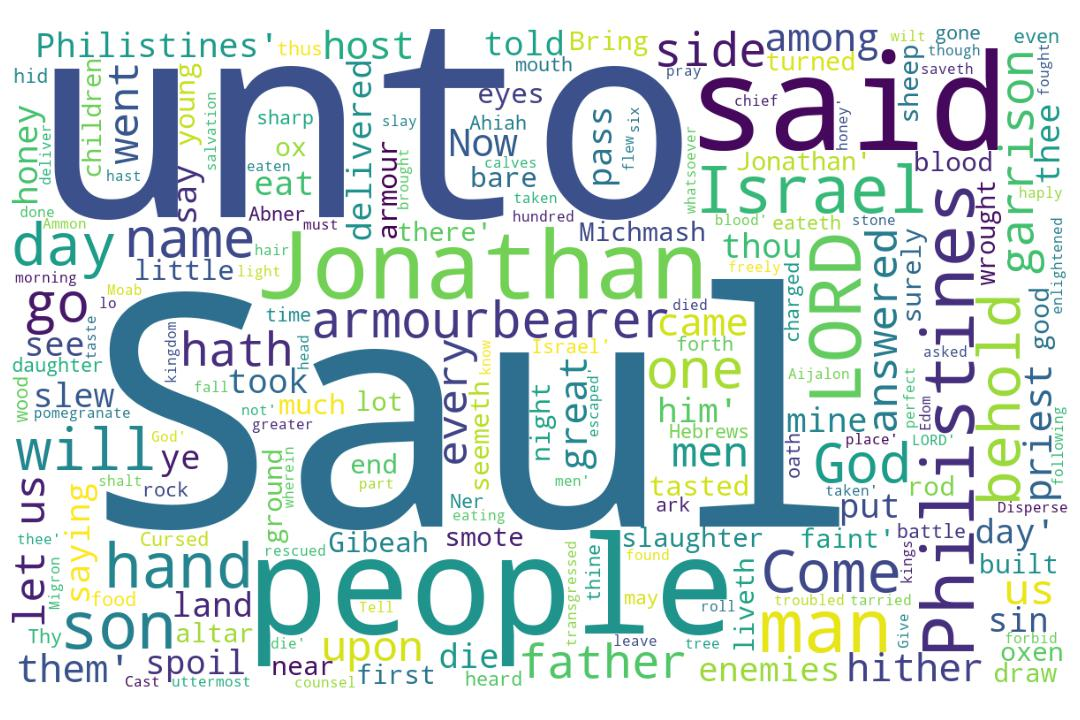
\includegraphics[width=\linewidth]{09OT-1Samuel/1Samuel14-WordCloud.jpg}
  \caption{1 Samuel 14 Word Cloud}
  \label{fig:1 Samuel 14 Word Cloud}
\end{figure}




\marginpar{\scriptsize \centering \fcolorbox{bone}{lime}{\textbf{SAUL, JONATHAN, AND}}\\\fcolorbox{bone}{lime}{\textbf{PHILISTINES}}\\ (1 Samuel 14:1--52) 
\begin{compactenum}[I.][8]
    \item  A \textbf{Shrewd Decision} \index[scripture]{1Samuel!1Sa 14:01} (1Sa 14:1) 
    \item   \textbf{Serious Deliverance} \index[scripture]{1Samuel!1Sa 14:10} \index[scripture]{1Samuel!1Sa 14:12}\index[scripture]{1Samuel!1Sa 14:48} (1Sa 14:10, 12, 48) 
    \item  \textbf{Self Destruction} \index[scripture]{1Samuel!1Sa 14:20} (1Sa 14:20) 
    \item  A \textbf{Stupid Directive} \index[scripture]{1Samuel!1Sa 14:24} (1Sa 14:24) 
    \item  \textbf{So Much Distress} \index[scripture]{1Samuel!1Sa 14:24} (1Sa 14:24) 
    \item \textbf{Salvation Dispensed} \index[scripture]{1Samuel!1Sa 14:45} (1Sa 14:45) 
    \item \textbf{Spoilers Destroyed} \index[scripture]{1Samuel!1Sa 14:48} (11Sa 14:48) 
\end{compactenum}}

%%%%%%%%%%%%%%%%%%%%%%%%%%%%%%%%%%%%%%%
%%%%%%%%%%%%%%%%%%%%%%%%%%%%%%%%%%%%%%%
\footnote{\textcolor[cmyk]{0.99998,1,0,0}{\hyperlink{TOC}{Return to end of Table of Contents.}}}\footnote{\href{https://audiobible.com/bible/1_samuel_14.html}{\textcolor[cmyk]{0.99998,1,0,0}{1 Samuel 14 Audio}}}\textcolor[cmyk]{0.99998,1,0,0}{Now it came to pass upon a day, that Jonathan the son of Saul said unto the young man that bare his armour, Come, and \fcolorbox{bone}{lime}{let us go over} to the Philistines' garrison, that \emph{is} on the other side. But\fcolorbox{bone}{bone}{he}told not his father.}
[2] \textcolor[cmyk]{0.99998,1,0,0}{And Saul tarried in the uttermost part of Gibeah under a pomegranate tree which \emph{is} in Migron: and the people that \emph{were} with him \emph{were} about six hundred men;}
[3] \textcolor[cmyk]{0.99998,1,0,0}{And Ahiah, the son of Ahitub, I-chabod's brother, the son of Phinehas, the son of Eli, the LORD'S priest in Shiloh, wearing an ephod. And the people knew not that Jonathan was gone.}\\
\\
\P \textcolor[cmyk]{0.99998,1,0,0}{And between the passages, by which Jonathan sought to go over unto the Philistines' garrison, \emph{there} \emph{was} a sharp rock on the one side, and a sharp rock on the other side: and the name of the one \emph{was} Bozez, and the name of the other Seneh.}
[5] \textcolor[cmyk]{0.99998,1,0,0}{The forefront of the one \emph{was} situate northward over against Michmash, and the other southward over against Gibeah.}
[6] \textcolor[cmyk]{0.99998,1,0,0}{And Jonathan said to the young man that bare his armour, Come, and let us go over unto the garrison of these uncircumcised: it may be that the LORD will work for us: for \emph{there} \emph{is} no restraint to the LORD to save by many or by few.}
[7] \textcolor[cmyk]{0.99998,1,0,0}{And his armourbearer said unto him, Do all that \emph{is} in thine heart: turn thee; behold, I \emph{am} with thee according to thy heart.}
[8] \textcolor[cmyk]{0.99998,1,0,0}{Then said Jonathan, Behold, we will pass over unto \emph{these} men, and we will discover ourselves unto \fcolorbox{bone}{bone}{them}.}
[9] \textcolor[cmyk]{0.99998,1,0,0}{If they say thus unto us, Tarry until we come to you; then we will stand still in our place, and will not go up unto \fcolorbox{bone}{bone}{them}.}
[10] \textcolor[cmyk]{0.99998,1,0,0}{But if they say thus, Come up unto us; then we will go up: for the LORD hath \fcolorbox{bone}{lime}{delivered} \fcolorbox{bone}{bone}{them} into our hand: and this \emph{shall} \emph{be} a sign unto us.}
[11] \textcolor[cmyk]{0.99998,1,0,0}{And both of \fcolorbox{bone}{bone}{them} discovered themselves unto the garrison of \fcolorbox{bone}{bone}{the Philistines} : and \fcolorbox{bone}{bone}{the Philistines}  said, Behold, the Hebrews come forth out of the holes where they had hid themselves.}
[12] \textcolor[cmyk]{0.99998,1,0,0}{And the men of the garrison answered Jonathan and his armourbearer, and said, Come up to us, and we will shew you a thing. And Jonathan said unto his armourbearer, Come up after me: for the LORD hath \fcolorbox{bone}{lime}{delivered} \fcolorbox{bone}{bone}{them} into the hand of Israel.}
[13] \textcolor[cmyk]{0.99998,1,0,0}{And Jonathan climbed up upon his hands and upon his feet, and his armourbearer after him: and they fell before Jonathan; and his armourbearer slew after him.}
[14] \textcolor[cmyk]{0.99998,1,0,0}{And that first slaughter, which Jonathan and his armourbearer made, was about twenty men, within as it were an half acre of land, \emph{which} a yoke \emph{of} \emph{oxen} \emph{might} \emph{plow}.}
[15] \textcolor[cmyk]{0.99998,1,0,0}{And there was trembling in the host, in the field, and among all the people: the garrison, and the spoilers, they also trembled, and the earth quaked: so it was a very great trembling.}
[16] \textcolor[cmyk]{0.99998,1,0,0}{And the watchmen of Saul in Gibeah of Benjamin looked; and, behold, the multitude melted away, and they went on beating down \emph{one} \emph{another}.}
[17] \textcolor[cmyk]{0.99998,1,0,0}{Then said Saul unto the people that \emph{were} with him, Number now, and see who is gone from us. And when they had numbered, behold, Jonathan and his armourbearer \emph{were} not \emph{there}.}\\
\\
\P \textcolor[cmyk]{0.99998,1,0,0}{And Saul said unto Ahiah, Bring hither the ark of God. For the ark of God was at that time with the children of Israel.}
[19] \textcolor[cmyk]{0.99998,1,0,0}{And it came to pass, while Saul talked unto the priest, that the noise that \emph{was} in the host of \fcolorbox{bone}{bone}{the Philistines}  went on and increased: and Saul said unto the priest, Withdraw thine hand.}
[20] \textcolor[cmyk]{0.99998,1,0,0}{And Saul and all the people that \emph{were} with him assembled themselves, and they came to the battle: and, behold, every man's sword was \fcolorbox{bone}{lime}{against his fellow}, \emph{and} \emph{there} \emph{was} a very great discomfiture.}
[21] \textcolor[cmyk]{0.99998,1,0,0}{Moreover the Hebrews \emph{that} were with \fcolorbox{bone}{bone}{the Philistines}  before that time, which went up with \fcolorbox{bone}{bone}{them} into the camp \emph{from} \emph{the} \emph{country} round about, even they also \emph{turned} to be with the Israelites that \emph{were} with Saul and Jonathan.}
[22] \textcolor[cmyk]{0.99998,1,0,0}{Likewise all the men of Israel which had hid themselves in mount Ephraim, \emph{when} they heard that \fcolorbox{bone}{bone}{the Philistines}  fled, even they also followed hard after \fcolorbox{bone}{bone}{them} in the battle.}
[23] \textcolor[cmyk]{0.99998,1,0,0}{So the LORD saved Israel that day: and the battle passed over unto Beth-aven.}\\
\\
\P \textcolor[cmyk]{0.99998,1,0,0}{And the men of Israel were \fcolorbox{bone}{lime}{distressed} that day: for Saul had adjured the people, saying, \fcolorbox{bone}{lime}{Cursed \emph{be}} the man that eateth \emph{any} food until evening, that I may be avenged on mine enemies. So none of the people tasted \emph{any} food.}
[25] \textcolor[cmyk]{0.99998,1,0,0}{And all \emph{they} \emph{of} the land came to a wood; and there was honey upon the ground.}
[26] \textcolor[cmyk]{0.99998,1,0,0}{And when the people were come into the wood, behold, the honey dropped; but no man put his hand to his mouth: for the people feared the oath.}
[27] \textcolor[cmyk]{0.99998,1,0,0}{But Jonathan heard not when his father charged the people with the oath: wherefore\fcolorbox{bone}{bone}{he}put forth the end of the rod that \emph{was} in his hand, and dipped it in an honeycomb, and put his hand to his mouth; and his eyes were enlightened.}
[28] \textcolor[cmyk]{0.99998,1,0,0}{Then answered one of the people, and said, Thy father straitly charged the people with an oath, saying, Cursed \emph{be} the man that eateth \emph{any} food this day. And the people were faint.}
[29] \textcolor[cmyk]{0.99998,1,0,0}{Then said Jonathan, My father hath troubled the land: see, I pray you, how mine eyes have been enlightened, because I tasted a little of this honey.}
[30] \textcolor[cmyk]{0.99998,1,0,0}{How much more, if haply the people had eaten freely to day of the spoil of their enemies which they found? for had there not been now a much greater slaughter among \fcolorbox{bone}{bone}{the Philistines} ?}
[31] \textcolor[cmyk]{0.99998,1,0,0}{And they smote \fcolorbox{bone}{bone}{the Philistines}  that day from Michmash to Aijalon: and the people were very faint.}
[32] \textcolor[cmyk]{0.99998,1,0,0}{And the people flew upon the spoil, and took sheep, and oxen, and calves, and slew \emph{them} on the ground: and the people did eat \emph{them} with the blood.}\\
\\
\P \textcolor[cmyk]{0.99998,1,0,0}{Then they told Saul, saying, Behold, the people sin against the LORD, in that they eat with the blood. And\fcolorbox{bone}{bone}{he}said, Ye have transgressed: roll a great stone unto me this day.}
[34] \textcolor[cmyk]{0.99998,1,0,0}{And Saul said, Disperse yourselves among the people, and say unto \fcolorbox{bone}{bone}{them}, Bring me hither every man his ox, and every man his sheep, and slay \emph{them} here, and eat; and sin not against the LORD in eating with the blood. And all the people brought every man his ox with him that night, and slew \emph{them} there.}
[35] \textcolor[cmyk]{0.99998,1,0,0}{And Saul built an altar unto the LORD: the same was the first altar that\fcolorbox{bone}{bone}{he}built unto the LORD.}\\
\\
\P \textcolor[cmyk]{0.99998,1,0,0}{And Saul said, Let us go down after \fcolorbox{bone}{bone}{the Philistines}  by night, and spoil \fcolorbox{bone}{bone}{them} until the morning light, and let us not leave a man of \fcolorbox{bone}{bone}{them}. And they said, Do whatsoever seemeth good unto thee. Then said the priest, Let us draw near hither unto God.}
[37] \textcolor[cmyk]{0.99998,1,0,0}{And Saul asked counsel of God, Shall I go down after \fcolorbox{bone}{bone}{the Philistines} ? wilt thou deliver \fcolorbox{bone}{bone}{them} into the hand of Israel? But\fcolorbox{bone}{bone}{he}answered him not that day.}
[38] \textcolor[cmyk]{0.99998,1,0,0}{And Saul said, Draw ye near hither, all the chief of the people: and know and see wherein this sin hath been this day.}
[39] \textcolor[cmyk]{0.99998,1,0,0}{For, \emph{as} the LORD liveth, which saveth Israel, though it be in Jonathan my son,\fcolorbox{bone}{bone}{he}shall surely die. But \emph{there} \emph{was} not a man among all the people \emph{that} answered him.}
[40] \textcolor[cmyk]{0.99998,1,0,0}{Then said\fcolorbox{bone}{bone}{he}unto all Israel, Be ye on one side, and I and Jonathan my son will be on the other side. And the people said unto Saul, Do what seemeth good unto thee.}
[41] \textcolor[cmyk]{0.99998,1,0,0}{Therefore Saul said unto the LORD God of Israel, Give a perfect \emph{lot}. And Saul and Jonathan were taken: but the people escaped.}
[42] \textcolor[cmyk]{0.99998,1,0,0}{And Saul said, Cast \emph{lots} between me and Jonathan my son. And Jonathan was taken.}
[43] \textcolor[cmyk]{0.99998,1,0,0}{Then Saul said to Jonathan, Tell me what thou hast done. And Jonathan told him, and said, I did but taste a little honey with the end of the rod that \emph{was} in mine hand, \emph{and}, lo, I must die.}
[44] \textcolor[cmyk]{0.99998,1,0,0}{And Saul answered, God do so and more also: for thou shalt surely die, Jonathan.}
[45] \textcolor[cmyk]{0.99998,1,0,0}{And the people said unto Saul, Shall Jonathan die, who hath wrought this great salvation in Israel? God forbid: \emph{as} the LORD liveth, there shall not one hair of his head fall to the ground; for\fcolorbox{bone}{bone}{he}hath wrought with God this day. So the people \fcolorbox{bone}{lime}{rescued Jonathan}, that\fcolorbox{bone}{bone}{he}died not.}
[46] \textcolor[cmyk]{0.99998,1,0,0}{Then Saul went up from following \fcolorbox{bone}{bone}{the Philistines} : and \fcolorbox{bone}{bone}{the Philistines}  went to their own place.}\\
\\
\P \textcolor[cmyk]{0.99998,1,0,0}{So Saul took the kingdom over Israel, and fought against all his enemies on every side, against Moab, and against the children of Ammon, and against Edom, and against the kings of Zobah, and against \fcolorbox{bone}{bone}{the Philistines} : and whithersoever\fcolorbox{bone}{bone}{he}turned himself,\fcolorbox{bone}{bone}{he}vexed \emph{them}.}
[48] \textcolor[cmyk]{0.99998,1,0,0}{And\fcolorbox{bone}{bone}{he}gathered an host, and smote the Amalekites, and \fcolorbox{bone}{lime}{delivered} Israel out of the hands of \fcolorbox{bone}{bone}{them} that spoiled \fcolorbox{bone}{bone}{them}.}
[49] \textcolor[cmyk]{0.99998,1,0,0}{Now the sons of Saul were Jonathan, and Ishui, and Melchi-shua: and the names of his two daughters \emph{were} \emph{these}; the name of the firstborn Merab, and the name of the younger Michal:}
[50] \textcolor[cmyk]{0.99998,1,0,0}{And the name of Saul's wife \emph{was} Ahinoam, the daughter of Ahimaaz: and the name of the captain of his host \emph{was} Abner, the son of Ner, Saul's uncle.}
[51] \textcolor[cmyk]{0.99998,1,0,0}{And Kish \emph{was} the father of Saul; and Ner the father of Abner \emph{was} the son of Abiel.}
[52] \textcolor[cmyk]{0.99998,1,0,0}{And there was sore war against \fcolorbox{bone}{bone}{the Philistines}  all the days of Saul: and when Saul saw any strong man, or any valiant man,\fcolorbox{bone}{bone}{he}took him unto him.}